
\section{Introducción}


%%%%%%------Descripción del juego------%%%%%%
\subsection{Descripción del juego}
\begin{frame}
  \frametitle{\insertsection}
  \framesubtitle{\hskip30pt \insertsubsection}

  \begin{block}{Hundir la flota. \em{Battleship}}
    \begin{itemize}
      \item\uncover<1->{Juego tradicional de guerra de estrategia (y suerte) por turnos.}
      \item\uncover<2->{Los dos jugadores colocan su flota en su tablero de forma secreta al contrincante.}
      \item\uncover<3->{Cada jugador en su turno intenta hundir los barcos del contrincante.}
      \item\uncover<4->{El objetivo es \textcolor{blue}{\em{Hundir la flota}} del contrincante.}
    \end{itemize}

  \end{block}
 
\end{frame}

\begin{frame}

  \begin{figure}
    \scalebox{0.2}{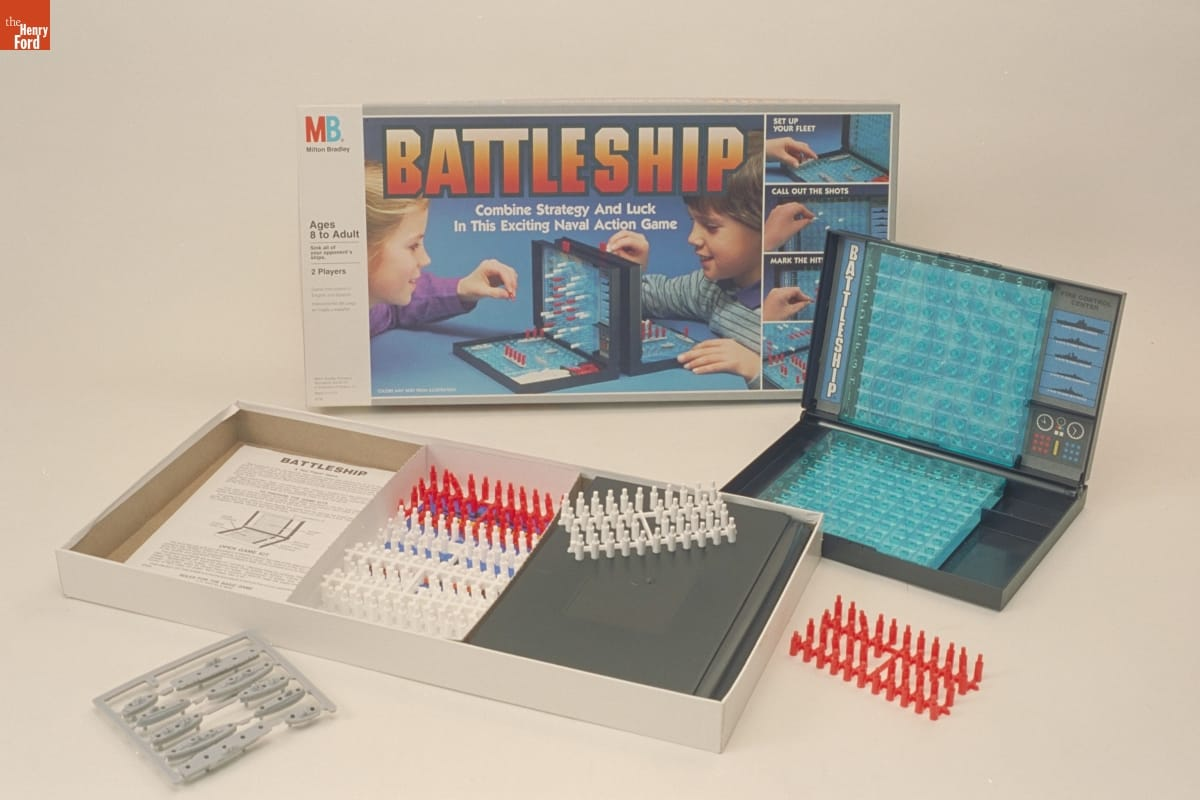
\includegraphics{imagenes/BattleShipOriginal.jpg}}
    \caption{Juego de mesa de hundir la flota. Año: 1980}
\end{figure}
\end{frame}


%%%%%%------Historia-----%%%%%%
\subsection{Historia}

\begin{frame}
  \frametitle{\insertsection}
  \framesubtitle{\hskip30pt \insertsubsection}

\begin{block}{Orígenes}
  \begin{itemize}
    \item\uncover<1->{Su posible origen está en el juego francés \textcolor{darkcerulean}{\em{L'Attaque}}\\ (publ. 	Hermance Edan, 1909)}
    \item\uncover<2->{La primera versión comercializada, \textcolor{orange}{\textit{Salvo}}, fue en 1931 por \textit{Starex Company.}}
    \item\uncover<3->{En 1967, \textcolor{blue}{Milton Bradley Company}, introduce una versión con tableros, barcos y otros elementos de plástico.}
    %\item En la actualidad, existen múltiples versiones digitales o en juegos de mesa.
  \end{itemize}
\end{block}

\end{frame}


\begin{frame}

  \begin{figure}
    \scalebox{0.55}{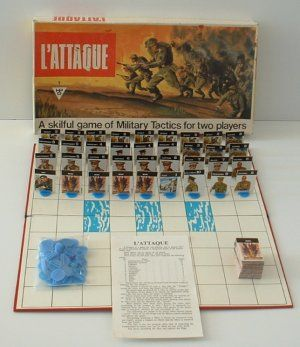
\includegraphics{imagenes/Lattaque.jpg}}
    \caption{Juego de mesa \em{L'Attaque}. Año: 1909}
  \end{figure}
\end{frame}

\begin{frame}

  \begin{figure}
    \scalebox{0.2}{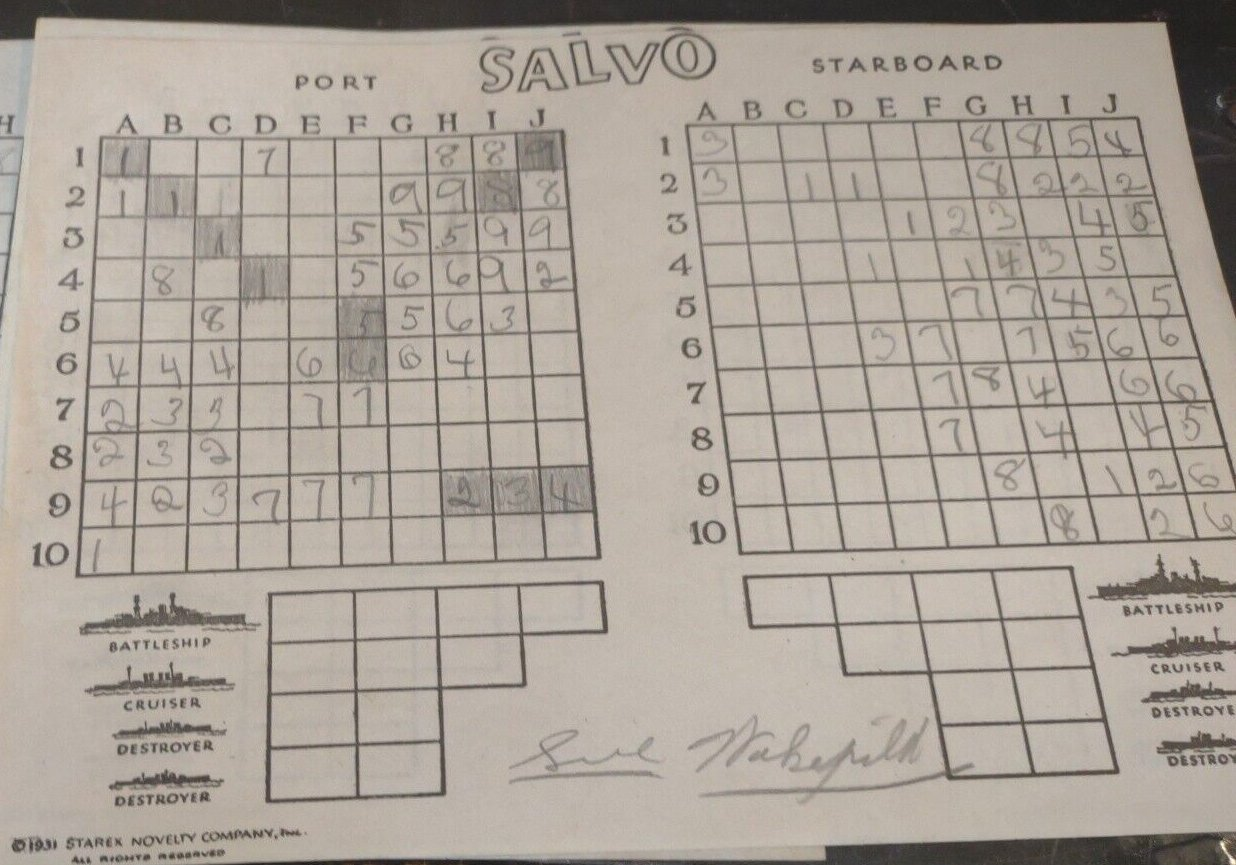
\includegraphics{imagenes/salvo2.jpg}}
    \caption{Juego de mesa \em{Salvo}. Año: 1931}
  \end{figure}
\end{frame}

\begin{frame}

  \begin{figure}
    \scalebox{0.6}{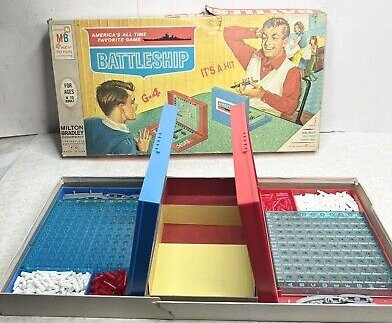
\includegraphics{imagenes/milton1967.jpg}}
    \caption{Juego de mesa \em{Battleship}. Año: 1967}
  \end{figure}
\end{frame}

\begin{frame}
  \frametitle{\insertsection}
  \framesubtitle{\hskip30pt \insertsubsection}

  \begin{block}{Evolución}

  \begin{itemize}
    \item\uncover<1->{En 1977, Milton lanza la primera versión computarizada: \textcolor{blue}{\textit{Electronic Battleship.}}}
    \item\uncover<2->{En 1984, \textcolor{orange}{Hasbro} adquiere Milton Bradley Company, y por tanto los derechos de \textit{Battleship}}
    \item\uncover<3->{La \textcolor{blue}{versión de Milton} es la que se ha expandido globalmente y la más conocida hasta hoy. }
    \item\uncover<4->{Se han creado múltiples variantes, desde juegos de mesa hasta digitales.}
   
  \end{itemize}
  \end{block}
\end{frame}

\begin{frame}

  \begin{figure}
    \scalebox{0.4}{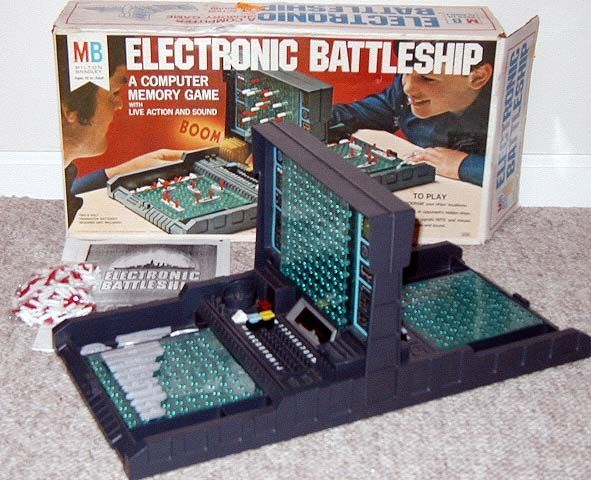
\includegraphics{imagenes/electronicBattleship.jpg}}
    \caption{Primera versión computarizada de \em{Battleship}. Año: 1977}
  \end{figure}
\end{frame}

\begin{frame}

  \begin{figure}
    \scalebox{0.23}{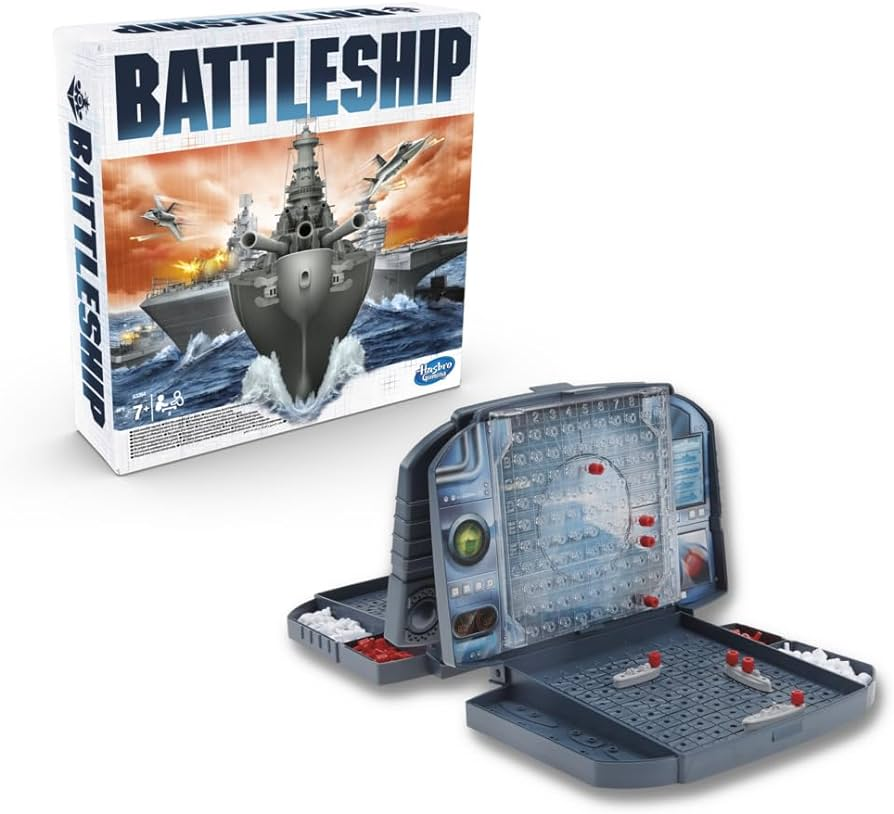
\includegraphics{imagenes/battleshipHasbro.jpg}}
    \caption{Versión actual de \em{Battleship} de Hasbro.}
  \end{figure}
\end{frame}

